% Latex multinotes package
% Test file for lecture notes

% Toggle the following options to see their effect

%\PassOptionsToPackage{blanks}{multinotes}
%\PassOptionsToPackage{blankproofs}{multinotes}
%\PassOptionsToPackage{noproofs}{multinotes}
%\PassOptionsToPackage{blankanswers}{multinotes}
%\PassOptionsToPackage{noanswers}{multinotes}

%------------------------------------------------
\documentclass{article}
%------------------------------------------------

\usepackage{../multinotes}

% multinotes options
\textcolour{black}
\backgroundcolour{yellow!4}
\proofcolour{blue}
\answercolour{red}
\showcolour{purple}

\framedblankboxes
\framedproofs
\framedanswers
\setboxrule{0.5pt}

\setstretchfactor{1.2} 
\setimagestretchfactor{1}

% layout
\usepackage[margin=20mm]{geometry}
\setlength{\parindent}{0ex}
\setlength{\parskip}{2ex}

% images
\usepackage{graphicx}
\usepackage{caption}
\usepackage{subfigure}
\graphicspath{{./figures/}}
\DeclareGraphicsExtensions{.png}

% theorems
\usepackage{amsthm}
\theoremstyle{definition}
\newtheorem{example}{Example}

% hyperref
\usepackage[hidelinks]{hyperref}
\setcounter{tocdepth}{2}

% misc
\usepackage{lipsum}
\usepackage{fancyvrb}


% tt backslash for use in section titles 
\newcommand{\vbs}{\char`\\}

% meta info
\title{Typesetting lecture notes with {\tt multinotes.sty}}
\author{DE}

%------------------------------------------------
\begin{document}
\maketitle

\tableofcontents
%\listof{video}{List of Videos}

\newpage

%------------------------------------------------
\section{Options}
%------------------------------------------------

The following package options are available.
\begin{table}[htb]
\renewcommand{\arraystretch}{1.3}
\addtolength{\tabcolsep}{2ex}
\begin{tabular}{lll}
\hline\hline
Option				& Effect \\
\hline
{\tt blanks}		& \verb+\blank+ macros and \verb+blankbox+ environments replaced by whitespace \\
{\tt noproofs}		& \verb+\prf+ macros and \verb+proof+ environments excluded \\
{\tt blankproofs}	& \verb+\prf+ macros and \verb+proof+ environments replaced by whitespace \\
{\tt noanswers}		& \verb+\ans+ macros and \verb+answer+ environments excluded \\
{\tt blankanswers}	& \verb+\ans+ macros and \verb+answer+ environments replaced by whitespace \\
{\tt nosketchboxes}	& \verb+sketchbox+ environments excluded \\
\hline\hline
\end{tabular}
\end{table}

The following style commands are available.
\begin{table}[htb]
\renewcommand{\arraystretch}{1.3}
\addtolength{\tabcolsep}{2ex}
\begin{tabular}{lll}
\hline\hline
Command							& \hspace{0.3\textwidth}\mbox{}\\
\hline
\verb+\textcolour{}+			&  set text colour\\
\verb+\backgroundcolour{}+		&  set background colour \\
\verb+\showcolour{}+			&  set text colour of blank boxes\\
\verb+\proofcolour{}+			&  set text colour of proofs \\
\verb+\answercolour{}+			&  set text colour of answer boxes \\
\hline
\verb+\framedblankboxes+		&  framed blankboxes \\
\verb+\framedproofs+			&  framed proofs\\
\verb+\framedanswers+			&  framed anwers\\
\verb+\setboxrule{}+			&  set frame thickness\\
\hline
\verb+\setstretchfactor{}+		&  to accomodate handwriting in blank boxes\\
\verb+\setimagestretchfactor{}+	&  to accomodate hand-drawing in blank boxes\\
\hline\hline
\end{tabular}
\end{table}

%------------------------------------------------
\section{Inline boxes}
%------------------------------------------------
The following macros replace their content by whitespace in response to differnet options. These can be used for partial handouts to accompany lectures or videos, or for missing-word exercises etc.
\begin{itemize}
\item \verb+\blank{...}+ is emptied by the {\tt blanks} option.
\item \verb+\fillbox{...}+ is emptied by {\tt blankanswers} and {\tt noanswers}.
\item \verb+\ans{...}+ is emptied by {\tt blankanswers} and removed by {\tt noanswers}.
\item \verb+\prf{...}+ is emptied by {\tt blankproofs} and removed by {\tt noproofs}.
\end{itemize}

%----------------------------------------
\subsection{\tt\vbs blank}
%----------------------------------------
Inline text replaced by whitespace by the {\tt blanks} option.

\begin{Verbatim}[frame=single]
Here is some \blank{text} to be hidden.
\end{Verbatim}
Here is some \blank{text} to be hidden.


%----------------------------------------
\subsection{\tt\vbs fillbox}
%----------------------------------------
Similar to \verb+\blank+ but controlled by \verb+blankanswers+.

\begin{Verbatim}[frame=single]
Roses are \fillbox{red}, violets are \fillbox{blue}.
\end{Verbatim}
Roses are \fillbox{red}, violets are \fillbox{blue}.

%----------------------------------------
\subsection{\tt\vbs ans}
%----------------------------------------
Similar to \verb+\fillbox+ but also controlled by the \verb+noanswers+ option.
%\begin{itemize}
%\item {\tt blankanswers} replaces the content by blank space. 
%\item {\tt noanswers} removes it completely.
%\end{itemize}

\begin{Verbatim}[frame=single]
What is $7\times 8$? \ans{54}
\end{Verbatim}
What is $7\times 8$\,? \ans{54}

%----------------------------------------
\subsection{\tt\vbs prf}
%----------------------------------------
Similar to \verb+\ans+ but controlled by \verb+blankproofs+ and \verb+noproofs+.
%\begin{itemize}
%\item {\tt blankproofs} replaces the content by blank space. 
%\item {\tt noproofs} removes it completely.
%\end{itemize}

\begin{Verbatim}[frame=single]
Thm: $\sin^2\theta+\cos^2\theta=1$. \prf{This follows by Pythagoras' theorem.}
\end{Verbatim}
Thm: $\sin^2\theta+\cos^2\theta=1$. \prf{This follows by Pythagoras' theorem.}



%------------------------------------------------
\section{Display boxes}
%------------------------------------------------
%The following environments replace displayed content by whitespace. The \verb+proof+ and \verb+answer+ environments can also be removed entirely (courtesy of the \verb+comment+ package).
\begin{itemize}
\item \verb+\begin{blankbox}...\end{blankbox}+ is controlled by the \verb+blank+ option.
\item \verb+\begin{proof}...\end{proof}+ is controlled by \verb+blankproofs+ and \verb+noproofs+.
\item \verb+\begin{answer}...\end{answer}+ is controlled by \verb+blankanswers+ and \verb+noanswers+.
\end{itemize}

%----------------------------------------
\subsection{The {\tt blankbox} environment}
%----------------------------------------

\subsubsection{A simple {\tt blankbox}}

\begin{Verbatim}[frame=single]
\begin{blankbox}
\lipsum[1]
\end{blankbox}
\end{Verbatim}
\begin{blankbox}
\lipsum[1]
\end{blankbox}

\subsubsection{A {\tt blankbox} with an optional title}

\begin{Verbatim}[frame=single]
\begin{blankbox}[\sl Some ideas]
\lipsum[2]
\end{blankbox}
\end{Verbatim}
\begin{blankbox}[\sl Some ideas]
\lipsum[2]
\end{blankbox}

\subsubsection{A {\tt blankbox} inside a theorem-like environment}

\begin{example}
If $X\sim\text{Poisson}(\lambda)$, compute $P(X\leq 2)$.
\begin{blankbox}[\sl Solution]
\[
P(X=k) = \displaystyle\frac{\lambda^ke^{-\lambda}}{k!}
\quad\text{so}\quad
P(X\leq 2) = \left(1 + \lambda + \frac{\lambda^2}{2}\right)e^{-\lambda}.
\]
\end{blankbox}
\end{example}
\begin{Verbatim}[frame=single]
\begin{example}
If $X\sim\text{Poisson}(\lambda)$, compute $P(X\leq 2)$.
\begin{blankbox}[\sl Solution]
\[
P(X=k) = \displaystyle\frac{\lambda^ke^{-\lambda}}{k!}
\quad\text{so}\quad
P(X\leq 2) = \left(1 + \lambda + \frac{\lambda^2}{2}\right)e^{-\lambda}.
\]
\end{blankbox}
\end{example}
\end{Verbatim}

%----------------------------------------
\subsection{The {\tt answer} environment}
%----------------------------------------
\begin{itemize}
\item {\tt blankanswers} replaces the contents by blank space. 
\item {\tt noanswers} removes it completely.
\end{itemize}

The {\tt noanswers} option is implemented using the {\tt comment} package. For it to work properly, the opening and closing commands \verb+\begin{answers}+ and \verb+\end{answers}+ must each appear on a line of its own, with no additional whitespace. This also applies to the \verb+proof+ environment with the {\tt noproofs} option.

Here is an answer (might be removed).
\begin{answer}
\lipsum[3]
\end{answer}

This is produced by the following code.
\begin{Verbatim}[frame=single]
\begin{answer}
\lipsum[3]
\end{answer}
\end{Verbatim}

% change proof title
Here is an answer with a custom title (might be removed).
\begin{answer}[\sl Answer to exercise 3]
\lipsum[4]
\qed
\end{answer}

This is produced by the following code.
\begin{Verbatim}[frame=single]
\begin{answer}[\sl Answer to exercise 3]
\lipsum[4]
\qed
\end{answer}
\end{Verbatim}

%----------------------------------------
\subsection{The {\tt proof} environment}
%----------------------------------------
\begin{itemize}
\item {\tt blankproofs} replaces the contents by blank space. 
\item {\tt noproofs} removes the proof completely.
\end{itemize}

Here is a proof (might be removed).
\begin{proof}
\lipsum[5]
\end{proof}

This is produced by the following code.
\begin{Verbatim}[frame=single]
\begin{proof}
\lipsum[5]
\end{proof}
\end{Verbatim}

% change proof title
Here is a proof with a custom title (might be removed).
\begin{proof}[\sl Proof of main theorem]
\lipsum[6]
\end{proof}

This is produced by the following code.
\begin{Verbatim}[frame=single]
\begin{proof}[\sl Proof of main theorem]
\lipsum[6]
\end{proof}
\end{Verbatim}

%------------------------------------------------
\section{Sketchboxes}
%------------------------------------------------
The \verb+sketchbox+ command produces an empty box for drawing sketches during live sessions. The mandatory argument determines the height of the box as a proportion of \verb+\textheight+. The optional argument provides a title for the box.

\sketchbox[Draw your sketch here]{0.15}

This is produced by the following code:
\begin{Verbatim}[frame=single]
\sketchbox[Draw your sketch here]{0.15}
\end{Verbatim}

%------------------------------------------------
\section{Videos}
%------------------------------------------------
The \verb+\includevideo+ macro and \verb+video+ environment are incorporated in anticipation of an effective LaTeX to HTML conversion method. For PDF output, video content is rendered as a simple hyperlink.

%----------------------------------------
\subsection{\tt\vbs includevideo}
%----------------------------------------
The \verb+\includevideo+ command mirrors \verb+\includegraphics+. 

\bigskip
\fbox{\centerline{\includevideo[scale=0.5]{https://youtu.be/wqGUwL0P6no}}}

\bigskip
This is produced by the following code:
\begin{Verbatim}[frame=single]
\includevideo[scale=0.5]{https://youtu.be/wqGUwL0P6no}
\end{Verbatim}

%----------------------------------------
\subsection{The {\tt video} environment}
%----------------------------------------

A new float called {\tt video} mimics the {\tt figure} and {\tt table} environments. These can be framed and captioned. A corresponding \verb+\listofvideos+ (suffix {\tt .lov}) can be included.

\begin{video}
\centering
\includevideo[scale=0.5]{https://youtu.be/wqGUwL0P6no}
\caption{Optimistic voices\label{vid:optimistic}}
\end{video}

This is produced by the following code:
\begin{Verbatim}[frame=single]
\begin{video}
\centering
\includevideo[scale=0.5]{https://youtu.be/wqGUwL0P6no}
\caption{Optimistic voices\label{vid:optimistic}}
\end{video}
\end{Verbatim}


%------------------------------------------------
\section{Images}
%------------------------------------------------

%----------------------------------------
\subsection{\tt\vbs includegraphics}
%----------------------------------------
\verb+\includegraphics{img}+ replaces \verb+img+ by whitespace whenever the {\tt blanks} option is set.


\begin{Verbatim}[frame=single]
\begin{blankbox}
\resizebox{0.3\textwidth}{!}{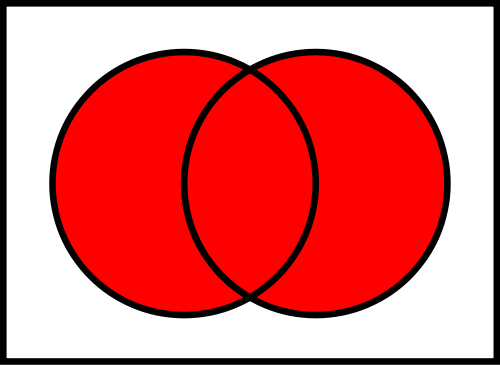
\includegraphics{AcupB}}
\end{blankbox}
\end{Verbatim}

\begin{blankbox}
\resizebox{0.3\textwidth}{!}{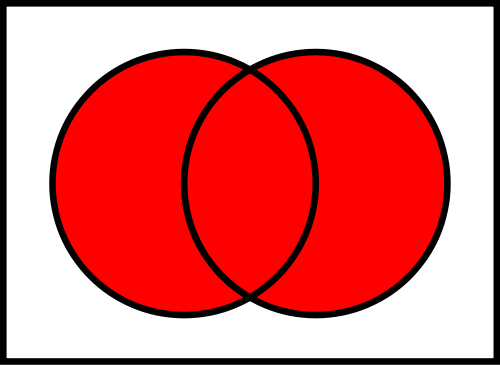
\includegraphics{AcupB}}
\end{blankbox}

%----------------------------------------
\subsection{\tt\vbs includetwographics}
%----------------------------------------

\verb+\includetwographics{img1}{img2}+ shows \verb+img2+ whenever {\tt blanks}, {\tt blankproofs} or {\tt blankanswers} is set, otherwise it shows \verb+img1+. This can be used to print partial images in handout notes and exercise sheets. 

\begin{Verbatim}[frame=single]
\begin{blankbox}
\resizebox{0.3\textwidth}{!}{\includetwographics[scale=1]{AcupB}{emptyset}}
\resizebox{0.3\textwidth}{!}{\includetwographics[scale=1]{AcapB}{emptyset}}
\resizebox{0.3\textwidth}{!}{\includetwographics[scale=1]{Acomp}{emptyset}}
\end{blankbox}
\end{Verbatim}

\begin{blankbox}
\resizebox{0.3\textwidth}{!}{\includetwographics[scale=1]{AcupB}{emptyset}}
\resizebox{0.3\textwidth}{!}{\includetwographics[scale=1]{AcapB}{emptyset}}
\resizebox{0.3\textwidth}{!}{\includetwographics[scale=1]{Acomp}{emptyset}}
\end{blankbox}


%----------------------------------------
\subsection{TikZ}
%----------------------------------------

% create random walk picture
\usetikzlibrary{math}
\usetikzlibrary{calc}
\tikzset{every picture/.style={line width=1pt}}
\tikzset{every picture/.append style={x=1cm,y=0.5cm}}
\tikzset{every picture/.append style={font=\Large}}
\pgfmathsetseed{\number\pdfrandomseed}
\tikzset{
	axes/.pic={
	\draw[help lines, color=gray!30, dashed] (-0.9,-9.9) grid (10.9,9.9);
	\draw[->,thick] (-1,0)--(11,0) node[right]{$t$};
	\draw[->,thick] (0,-10)--(0,10) node[above]{$x$};
	}
}
\tikzset{
	samplepaths/.pic={
		\foreach \c in {red, green, blue}
		    \draw [\c] (0,0) \foreach ~ in {0,...,10}{-- ++(1,{random(0,1)*2-1})};
	}
}
\tikzset{
    rwalk/.pic={
        \pic{axes};
        \pic{samplepaths};
    }
}

% tikz picture
%\begin{Verbatim}[frame=single]
%\resizebox{0.5\textwidth}{!}{\tikz\pic{rwalk};}
%\end{Verbatim}
%
%\begin{figure}[htb]
%\centering
%\resizebox{0.5\textwidth}{!}{\tikz\pic{rwalk};}
%\caption{A random walk!\label{fig:rwalk}}
%\end{figure}


% show 
Here is a tikz pcture in a blankbox. The \verb+\blanktikz+ command should make it disappear when the {\tt blanks} option is set.
\begin{Verbatim}[frame=single]
\begin{blankbox}
\blanktikz
\resizebox{0.5\textwidth}{!}{\tikz\pic{rwalk};}
\end{blankbox}
\end{Verbatim}

\showcolour{black}
\begin{blankbox}
\blanktikz
\resizebox{0.5\textwidth}{!}{\tikz\pic{rwalk};}
\end{blankbox}
%

%------------------------------------------------
\end{document}
%------------------------------------------------


